\documentclass{beamer}
\usetheme{default}

\title{Feedbackdashboard IJkingstoets}
\author{Jesse Hoobergs}
\begin{document}
\begin{frame}[plain]
    \maketitle
\end{frame}
%\begin{frame}
%	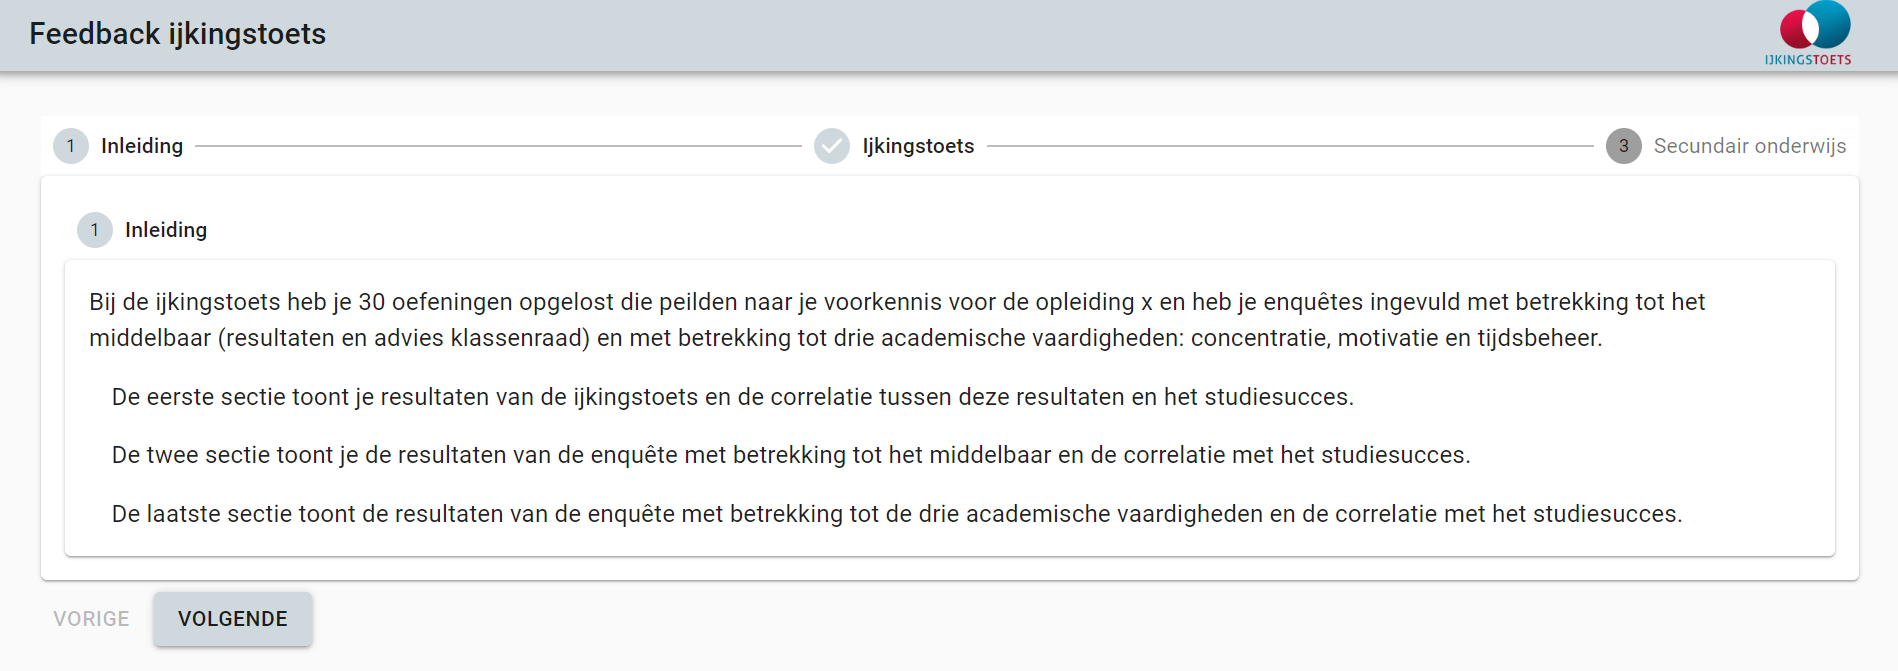
\includegraphics[scale=0.35]{overview}
%\end{frame}

\begin{frame}{Doel}
    \begin{block}{Feedbackdashboard}
        \begin{itemize}
            \item Genuanceerde feedback geven aan de deelnemer
            \item Elke deelnemer krijgt feedback toegespitst op zijn/haar exacte score.
        \end{itemize}
    \end{block}
    
    \begin{block}{Meeting}
            \begin{itemize}
                \item Uitleg over het dashboard
                \item Uitleg over het beheren van het dashboard
                \item Samen kijken naar mogelijke invulling
                \begin{itemize}
                \item Wat kan nog niet ?
                \end{itemize}
            \end{itemize}
        \end{block}
\end{frame}

\begin{frame}{Concept}
	\begin{itemize}
        \item Online feedbackdashboard
		\item Per sessie en per toets is er een aparte layout
			\begin{itemize}
				\item Layout bestaat uit 'stappen' en 'substappen'
				\item Elke van deze substappen bevat inhoud
                \item Deze inhoud kan 'variabelen' bevatten
                \item Deze inhoud kan 'visualisaties' bevatten
                \item Deze inhoud kan conditionele stukken bevatten
			\end{itemize}
        \item Aparte url per sessie van een toets: e.g /13/wb, /14/ir, \ldots 
	\end{itemize}
     \begin{block}{Huidige versie}
        \begin{itemize}
        \item \url{http://set-p-dsb-ijkingstoets-feedback-dashboard.cloud-ext.icts.kuleuven.be}
        \item Binnenkort: \url{https://feedback.ijkingstoets.be}
        \end{itemize}
      \end{block}
\end{frame}

\begin{frame}{Flow}
	\begin{enumerate}
        \item Deelnemer schrijft zich in voor de ijkingstoets
		\item Deelnemer doet mee aan de ijkingstoets
        \item Antwoordformulieren worden ingelezen via OMR
        \item De resultaten worden berekend via een script
        \begin{itemize}
            \item OMR files nodig
            \item 'config' file nodig
            \item file met juiste antwoorden per vraag nodig
            \item file met permutaties van vragen nodig bij meerdere vragenlijsten  
        \end{itemize}
        \item Data wordt toegevoegd aan het feedbackdashboard
        \item Feedback is beschikbaar
        \item Deelnemer krijgt een mail met rechtstreekse link naar zijn of haar feedback
	\end{enumerate}
\end{frame}

\begin{frame}{Tijdlijn}
    \begin{itemize}
        \item Voorbeeld wb toets tegen eind januari
        \item Wb toets in 2020
        \item Andere toetsen vanaf 2021 
    \end{itemize}
\end{frame}

\begin{frame}{Beheer}
Het wijzigen van de stappen, substappen, hun inhoud en volgorde gebeurt via de website
	\begin{itemize}
		\item Edit mode is enkel geactiveerd als je een speciale code ingeeft als 'ijkingstoetscode'
		\item 'Variabelen' kunnen gebruikt worden in de tekst om student-specifieke waarden te tonen (e.g score van student)
		\item 'Visualisaties' kunnen gebruikt worden in de tekst om grafieken toe te voegen etc
		\item Een stuk tekst kan conditioneel zijn, enkel getoond voor als aan een voorwaarde voldaan is (e.g enkel voor geslaagde student)
	\end{itemize}
\end{frame}

\begin{frame}{Verbeterpunten}
    \begin{itemize}
    \item Verbeteren visualisaties
    \begin{itemize}
        \item Meer visualisaties
            \begin{itemize}
                \item ...
            \end{itemize}
        \item Extra features bij bestaande
    \end{itemize}
    \item Meer variabelen
    \begin{itemize}
    \item ...
    \end{itemize}
    \item Moeilijk om layout in te vullen, als er geen data is
        \begin{itemize}
            \item Testcodes met fake data ? (Moet dan up to date blijven met inhoud toets etc)
        \end{itemize}
     \item \ldots
    \end{itemize}
\end{frame}

\end{document}
